\pdfcompresslevel9
\pdfdecimaldigits2
\pdfminorversion4

\documentclass[12pt,a4paper]{book}
\usepackage[bottom=2.5cm,top=3.5cm]{geometry}
%\usepackage{ngerman}
\usepackage[utf8]{inputenc}
\usepackage[T1]{fontenc}
\usepackage{graphicx}
\usepackage{colortbl}
\usepackage{ae}
\usepackage{amssymb}
\usepackage{amsmath}
\usepackage{amsthm}
\usepackage{multirow}
\usepackage{rotating}
\usepackage[margin=10pt,font=small,labelfont=bf]{caption}
\usepackage{listings}
\usepackage{microtype}

%\linespread{1.25}
\setlength{\parindent}{0pt}

\usepackage{fancyhdr}
\usepackage[
  	pdfstartview=FitH,   
  	pdffitwindow=true,
	pdftitle = "Models of Computation WiSe1011 UdS", % Sets the document information Title field
    pdfauthor = "Adrian Neumann", %Sets the document information Author field
  	colorlinks,
  	linkcolor=black,
  	anchorcolor=black,
  	citecolor=black,
  	urlcolor=black
]{hyperref}

\pagestyle{fancy}
\cfoot{\thepage}

\newsavebox{\footerlicence}
\sbox{\footerlicence}{
\includegraphics{./images/by-nc-sa}}

\rfoot{\usebox{\footerlicence}}
\fancyhead{}
\lfoot{Found a mistake? Write an e-mail!}

\definecolor{gruen}{rgb}{0.5,1,0.5}
\definecolor{rot}{rgb}{1,0.5,0.5}


\renewcommand{\footrulewidth}{0.4pt}
\renewcommand{\headrulewidth}{0pt}
\newcommand{\B}[0]{\mathbb{B}}
\newcommand{\N}[0]{\mathbb{N}}
\newcommand{\Z}[0]{\mathbb{Z}}
\newcommand{\Q}[0]{\mathbb{Q}}
\newcommand{\R}[0]{\mathbb{R}}
\newcommand{\C}[0]{\mathbb{C}}
\newcommand{\E}[0]{\mathbb{E}}
\newcommand{\im}[0]{\mathit{i}}
\newcommand{\kthings}[2]{{#1}_1,\ldots,{#1}_{#2}}
\newcommand{\nthings}[1]{\kthings{#1}{n}}
\newcommand{\norm}[1]{|\!|#1|\!|}
\newcommand{\rank}{\mbox{rank }}
\newcommand{\skal}[1]{\left\langle {#1} \right\langle}
\newcommand{\ok}{{\large \checkmark}}
\newcommand{\no}{{\large $\mathbb{\times}$}}
\newcommand{\nz}{\text{nz}}
\newcommand{\rup}[1]{\left\lceil #1 \right\rceil}
\renewcommand{\bar}{\overline}
\renewcommand{\arraystretch}{1.5}
\newcommand{\argmin}[1]{\underset{#1}{\operatorname{argmin}}}



\newcommand{\trans}[1]{{#1}^\text{\upshape \sffamily T}}
\newtheoremstyle{leplain} %name
    {2em} %above
    {2em} %below
    {} %body font
    {} %indent
    {\bfseries} %head font
    {:} %punctuation after head
    {0.5em} %space after head
    {} %head spec
\title{Models of Computation}
\author{Adrian Neumann \\ {\small \texttt{adrian\_neumann@gmx.de}}}


\date{}

\begin{document}
\frontmatter
\lstdefinelanguage{pseudocode}{
    morekeywords = {repeat, until, if, unless, while, for, return, break},
    sensitive = false,
    morecomment=[l]{//},
    morecomment=[s]{/*}{*/},
}
\lstset{language=pseudocode, basicstyle=\sffamily\small\slshape, commentstyle=\slshape\sffamily, keywordstyle=\upshape\bfseries, breaklines=true, mathescape=true, tabsize=2}


\theoremstyle{definition}
\newtheorem{Def}{Definition}[section]

\theoremstyle{leplain}
\newtheorem{ex}{Example}[section]
\newtheorem{pr}{Proof}[section]
\newtheorem{cor}{Corollary}[section]
\newtheorem{lem}{Lemma}[section]

\theoremstyle{theorem}
\newtheorem{thm}{Theorem}[section]



\maketitle
\thispagestyle{fancy}

\section*{Disclaimer}

Most likely this script is riddled with errors so take everything with an appropriate dose of salt. Send the author emails or patches if you find errors or have some clarifications. 

These notes are released under a Creative Commons Attribution--Noncommercial--Share-Alike licence. So you can do pretty much everything with them as long as you mention the original authors, don't sell your work and distribute it under an equivalent licence. Read the licence agreement for details. Although the licence does not request it the author would be happy if you noticed him should you decide to use this.

\section*{Thanks}
The following persons have contributed:

\begin{center}
\begin{tabular}{l|c}
Name & Corrections\\\hline
Aram Harutyunan & 11
Radu Curticapean & 20
\end{tabular}
\end{center}
\newpage

\mainmatter

\chapter{Distributed Computing}

\section{Introduction}

Many autonomous entities with their own hardware (memory, CPU) in a system that connects them through a network over which they can send messages to each other. The natural way to represent that is a graph. There are many models to describe different aspects of the system. They have to deal with the following issues:

\begin{enumerate}
\item Communication. Usually communication is very expensive, its cost dominates all other costs. Hence it is typically assumed that communication is the only cost that occurs.
\item Fault Tolerance. In large computer networks it's common that a few nodes fail during the computation. Robustness against this is desirable. Results should be reasonable even if single entities fail.
\item Locality. Networks change over time, communicating these changes to all nodes would be too costly. It's better to design algorithms that only rely on local information.
\item Synchronization. Individual entities can have different hardware and solve problems at different speeds. It's good if algorithms don't have to assume synchronous computation.
\item Symmetry breaking. Nodes have to be made distinguishable.
\end{enumerate}

\section{Vertex Coloring}

Given an undirected graph $G=(V,E)$ we want to find a colouring, i.e. an assignment of colours $c_v$ to the vertices $v\in V$, such that no two adjacent vertices have the same colour.

This is useful for symmetry breaking. For example cellphones that communicate with the same cell have to choose different frequencies.

We will assume that initially all nodes are equipped with a unique ID$\in [1,n]$. Typically each ID uses $O(\log n)$ bits. Obviously the IDs are a valid colouring. We want to try to use fewer colours, if possible the minimal number.

\begin{Def}[Chromatic Number] The chromatic number $\chi(X)$ of a graph is the minimal number of colours needed in any valid colouring of G.
\end{Def}

Computing the chromatic number is NP-complete. Hence we want to try to find some approximate solution.

A simple, sequential algorithm assigns colours greedily:

\begin{lstlisting}
Greedy(graph G)
while $\exists$ uncoloured vertex v
	colour v with min ([1,n] - colours(neighb(v)))
\end{lstlisting}

\begin{thm} The greedy algorithm stops after $n$ steps and produces a valid colouring and uses at most $\Delta(G)+1$ colours\footnote{$\Delta(G)$ is the maximal degree of the graph}.
\end{thm}

\begin{pr} It is clear that the algorithm stops in $n$ steps, since in each iteration the number of vertices decreases by one. 

Correctness is given by an inductive argument. During the execution the coloured subgraph is always valid, since we assign colours that don't occur in the neighbourhood.

Finally $\Delta(G)+1$ is an upper bound for the number of colours since there is always a free colour in the set $[1,\Delta(G)+1]$ 
\end{pr}

We want to construct a distributed algorithm that uses the same ideas to reduce the number of colours.

\begin{lstlisting}
First-Free(coloured G, vertex v)
	give v the smallest available colour
\end{lstlisting}

This algorithm can produce error if two adjacent vertices choose the colour at the same time under certain circumstances.

\begin{figure}
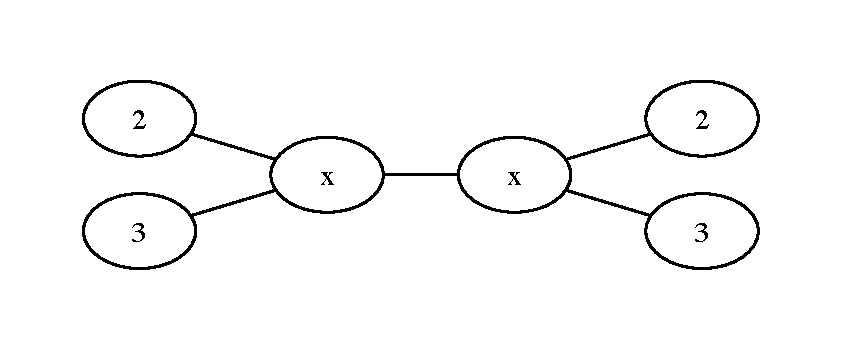
\includegraphics[width=0.5\linewidth]{./images/graph1}
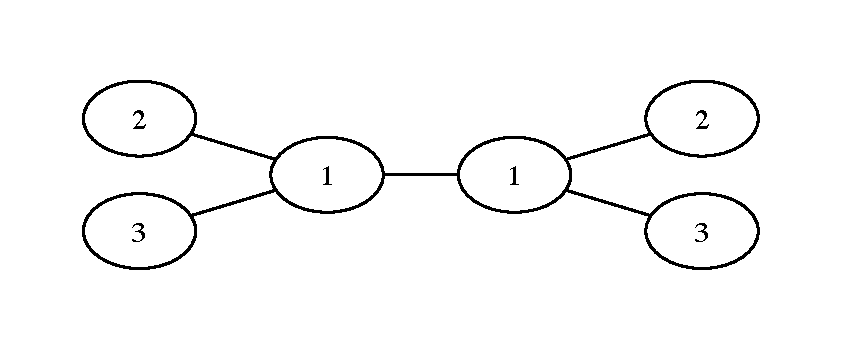
\includegraphics[width=0.5\linewidth]{./images/graph11}
\caption{If the nodes labelled with x have high IDs and choose simultaniously they produce an invalid colouring.}
%n1 2
%n2 x
%n3 3
%n4 10
%n5 2
%n6 3
%n1 -- n2
%n2 -- n3
%n2 -- n4
%n4 -- n5
%n4 -- n6
%
%n1 and n2 choose colours simultaniously, both get 1.
\end{figure}

It depends on the model how we can deal with this. Either we have the means for synchronisation, or we don't.

\begin{Def}[Synchronous Distributed Algorithm] During one unit of time an entity in a SDA can execute (in any order) the following things
\begin{itemize}
\item Perform local computations
\item Send messages
\item Receive messages
\end{itemize}

As long as they are of "reasonable" complexity
\end{Def}

In this model we can change the algorithm like this:

\begin{lstlisting}
Reduce
	send own ID to all neighbours
	receive IDs from all neighbours
	while $\exists$ uncolored vertex in the neighbourhood that has larger ID
		send "undecided" to all neighbours
		receive messages from neighbours
	colour thyself with First-Free
	send the colour to neighbours
\end{lstlisting}

\begin{thm} Reduce is correct, i.e. it produces a valid colouring after at most $n$ rounds. The number of colours used is upper bounded by $\Delta(G)+1$. 
\end{thm}

\begin{pr}
\end{pr}
\subsection{Colouring Trees}

In order to finde a faster algorithm we first look at a special case, trees. A tree is an acyclic connected graph. All trees are bipartite, and hence have chromatic number 2.

\begin{thm} $T$ is a tree implies $\chi(T)=2$ \end{thm}

\begin{pr} Let $v$ be a distinguished vertex, the root, in the tree. Colour $v$ red.  Colour every other vertex according to the distance from the root. If the distance is odd colour it blue, else red. Since there are no cycles in the graph, the coloring is valid.
\end{pr}

If we assume that the root knows that it's special we can construct the algorithm in figure \ref{alg:slow_tree_colour}

\begin{figure}[hbt]
\begin{lstlisting}
root: colour with red; send to all children
all except root: 
	wait for message
	if parent red
		colour blue
	else
		color red
	send colour to all children
\end{lstlisting}
\caption{Slow Tree Coloring}
\label{alg:slow_tree_colour}
\end{figure}


This algorithm isn't faster than the previous one, for degenerate trees. We also need to find a way to decide which node is the root. The latter problem is deferred to a later lecture.

Note that this algorithm doesn't need to operate in a synchronous environment. Every node waits for an event before it starts its computation. Event-driven algorithms can be implemented in asynchronous settings

\begin{Def}[Asynchronous DA] A asynchronous distributed algorithm has no access to a global clock and works event-driven.

Any sent message will arrive in finite time.
\end{Def}

There are different ways to assess the complexity of asynchronous algorithms (there are not bounds on the time a message takes). Typically we are interested in 

\begin{itemize}
\item Message Complexity: The number of messages sent
\item Time Complexity: Under the assumption that each message has delay 1, the time complexity is the length of the longest chain of interdependent messages.
\end{itemize}

\begin{thm} The asynchronous time complexity of algorithm \ref{alg:slow_tree_colour} is $\leq height(T)$ \end{thm}
\begin{pr} In the first round the root sends its colour to all neighbours. This costs one time unit. Argument follows from induction on the height\end{pr}

We now try to improve the algorithm to get a better runtime than $O(n)$. In fact we'll give an algorithm that is bounded by $O(\log^*n)$. We assume that all vertices know that the graph is a tree, a root is known and each node knows it's parent. How we find that information is again deferred to later

\begin{figure}[hbt]
\begin{lstlisting}
Let $c_v$ be ID(v)
repeat 
	send $c_v$ to all childrens
	if $v$ is the root then
		I=0
	else 
		let $c_p$ be the parent's colour
		I = smallest i s.t. bin$_i$($c_v$), bin$_i$($c_p$) differ
		$c_v$ = <bin(I),bin$_I$($c_v$)> //use $1+\log |c_v|$ bits  
		                                //even if I small
until |bin($c_v$)| does not change
\end{lstlisting}
\caption{6-colour}
\label{alg:6-colour}
\end{figure}

\begin{lem} Algorithm \ref{alg:6-colour} produces a valid colouring \end{lem}

\begin{pr} Since all IDs are different the colouring is valid in the first step. Now consider some iteration during the execution of the algorithm

Let $u$ be the parent of $w$. If $u$ finds $I_u$ and $w$ finds $I_w$ then the new colours are $c_u=<bin(I_u), bin_{I_u}(c_u)>, c_w<bin(I_w),b_{I_w}(c_w)>$. There are two cases

\begin{itemize}
\item $I_u\neq I_w$. Then the first part of the new colours differ. \ok
\item $I_u=I_w=I$. Then we have $b_I(c_u)\neq b_I(c_w)$, by the choice of $I$ \ok
\end{itemize}

So the colouring stays valid after each round.
\end{pr}

\begin{lem} Let $K_i$ be the number of bits in the representations of the colours in round $i$.

\begin{align*}
K_0 &= \left\lceil \log n\right\rceil\\
K_{i+1} &= 1+\left\lceil K_i\right\rceil
\end{align*}

\end{lem}

\begin{pr}
We have that $K_{i+1} < K_i$ as long as $K_i\geq 4$. If $K_i\in \{1,2,3\}$, we have $K_{i+1}=K_i$. Otherwise we can write $K_i=2^x\cdot y$, $x\in \N$, $y\in [1,2)$. Then we have

\[K_{i+1} = 1+\left\lceil \log(2^x\cdot y)\right\rceil = \begin{cases} 1+x & y=1\\ 2+x &y>1\end{cases}\]

So we have 

\[K_{i+1}<K_i \Leftrightarrow 2^x\cdot y > \begin{cases} 1+x & y=1\\ 2+x &y>1\end{cases}\]

check yourself that the exponential function on the left grows sufficiently fast for the claim to be true.
\end{pr}

\begin{thm} The final colouring uses at most 6 colours and stops after $O(\log^* n)$ rounds.\end{thm}

\begin{pr} Let $i$ be the final iteration. Since the algorithm stopped, we know $K_i=K_{i-1} \leq 3$. The colour is encoded as $<bin(I), bin_I(c)>$ since $I\leq 3$ we get only six possible colours.

For the running time we claim: $K_i\leq 2+ \left\lceil \log^{(i)} K_0 \right\rceil$. This can be proven by induction on $i$. 

$i=1$ \ok. $i\rightarrow i+1$:

\begin{align*}
K_{i+1}&= 1+\rup{\log K_i}\\
	&\leq 1+ \rup{\log(2+\rup{\log^{(i)}K_0})}\\
	&\leq 1+\rup{1+\log \rup{\log^{(i)} K_0}}\\
	&\leq 2+\rup{1+\log \rup{\log^{(i)} K_0}}\\
	&=\leq 2+\rup{1+\log \log^{(i)} K_0}\\
\end{align*}

If we choose $i=\log^*(K_0)$ we get $K_i\leq 4$ by definition of $\log^*$. Henc in round $\log^*(K_0)+2$ the algorithm will finish.
\end{pr}

Six colours isn't very satisfying for a bipartite graph, so we try to reduce the number of colours further.

\begin{figure}[hbt]
\begin{lstlisting}
root: choose a different colour
all others: take the old colour of parent
\end{lstlisting}
\caption{Shift-Down}
\label{alg:Shift-Down}
\end{figure}

Algorithm \ref{alg:Shift-Down} only takes one round.

\begin{lem} The colouring produced by algorithm \ref{alg:Shift-Down} is valid, if the intitial colouring is valid. Also, all siblings of a node have the same colour.\end{lem}

\begin{pr} Let $c'_u$ be the initial colours and $c_u$ be the new ones. Let $u_1\rightarrow u_2 \rightarrow u_3$ be a path in the tree. Then $c_{u_2}=c'_{u_1} \neq c_{u_3}=c'_{u_2}$. The root is also ok, since it chooses a fresh colour.\end{pr}

\begin{figure}[hbt]
\begin{lstlisting}
For $x\in \{3,4,5\}$
	Shift-Down
	All vertices coloured with $x$ call First-Free
\end{lstlisting}
\caption{6-to-3}
\label{alg:6-to-3}
\end{figure}

\begin{lem} The colouring produced by \ref{alg:6-to-3} is valid and contains $\leq 3$ colours.\end{lem}

\begin{pr} After the shift down, the neighbourhood of a vertex labelled with $x$ contains only two colours. The colour of the parent and the colours of the children. It can also not happen that two adjacent vertices call First-Free simultaniously, since then they would have had the same colour to begin with.\end{pr}

Finding a colouring with just 2 colours is not possible as fast.

\subsection{Lower Bounds}

\end{document}
